\documentclass[10pt]{article}
\usepackage{../../../local}
\usepackage{subcaption}
\usepackage{caption}
\usepackage{multirow}
\urlstyle{same}

\usepackage[style=numeric, sorting=none, maxnames=3]{biblatex}
\addbibresource{QIE.bib}

\newcommand{\classcode}{Physics 111B}
\newcommand{\classname}{Quantum Interference and Entanglement}
\renewcommand{\maketitle}{%
\hrule height4pt
\large{Eric Du \hfill \classcode}
\newline
\large{Lab 4} \Large{\hfill \classname \hfill} \large{\today}
\hrule height4pt \vskip .7em
\small{Header styling inspired by CS 70: \url{https://www.eecs70.org/}}
\normalsize
}
\linespread{1.2}
\begin{document}
	\maketitle

	\begin{abstract}
		In this experiment, we explore the phenomenon of quantum entanglement, and use its properties to
		violate the CHSH inequality, a historical result to definitively disprove the existence of hidden
		variable theories. The entanglement process is achieved using two beta barium borate (BBO) crystals,
		then vary the measurement basis using a series of half wave plates. Using a particular set of
		measurement bases, we are able to calculate a quantity \( S \), which is bounded above by \( |S| \leq
		2 \) if hidden variable theories exist. The violation of this inequality in our experiment confirms
		the lack of such theories, and confirms the nonlocal nature of quantum mechanics.
	\end{abstract}


	\section{Introduction}

	This report concerns the QIE experiment in the Physics 111B Experimentation
	Laboratory. In this report, we will begin by detailing the theoretical background
	for the phenomena, then analyze the data we collect to verify our theoretical
	results. 
	\section{Theory}

	In this section, we will go over all the requisite theory needed to complete this lab. First, we will
	briefly go over quantum states, measurement, and the CHSH inequality, which is the central focus of our
	experiment.  

	\subsection{Quantum States}
	In quantum mechanics, the fundamental building block we use to characterize particles is the \textit{quantum
	state} \( \ket*{\psi} \). For the purposes of our experiment, we will deal only with two-state systems,
	meaning that our state \( \ket*{\psi} \) only has two possible representations fundamentally, those being
	\( \ket*{0} \) and \( \ket*{1} \), or in our case, we will use \( \ket*{v} \) and \( \ket*{h} \) for
	reasons which will become obvious later. 

	One key property of quantum states, that are different than classical ones is that they need not exist
	purely in \( \ket*{v} \) or \( \ket*{h} \), but may exist in a \textit{linear combination} of these two
	states. That is, it is possible to find a particle in the state:
	\[
		\ket*{\psi} = \alpha \ket*{v} + \beta \ket*{h}
	\]
	In this representation, the coefficients \( \alpha, \beta \in \C \) represent the measurement
	probabilities -- that is, if we were to measure the state \( \ket*{\psi} \), the postulates of quantum
	mechanics says that the state now collapses into one of \( \ket*{v} \) and \( \ket*{h} \) (its
	constituent states), and the probability of either event occurring is given by \( |\alpha|^2 \) and \(
	|\beta|^2 \), respectively.

	The theory we've just described is complete for a single particle two-state system. In this lab, we will
	be dealing with two particles, so it will be useful to investigate how those states behave as well.
	When we have two non-interacting particles, due to the fact that one particle doesn't affect the
	other, then intuitively one expects that the behavior of one particle doesn't affect the other. From a
	probability theory standpoint, we call these two \textit{independent}. As with independent events, if we
	are to consider the joint probability distribution of two particles, then due to independence it means
	that the joint probability is just the product of the two probabilities. Because states are inherently
	vectors, then this definition changes from a simple product to a \textit{tensor product}, which is
	basically a fancy product symbol. We don't really need to worry too much about it. In essence, a
	two-particle state can be written as follows:
	\begin{equation}
		\label{state}
		\ket*{\psi} = \alpha \ket*{vh} + \beta \ket*{hh}
	\end{equation}
	where the way we read this is the exact same as the one-particle state: the probability of observing
	state \( \ket*{vh} \) is \( |\alpha|^2 \), and likewise for \( |\beta|^2 \). The state \( \ket*{vh} \) is
	really shorthand for \( \ket*{v} \otimes \ket*{h} \), and this means that the first particle is in the \(
	\ket*{v}\) state and the second is in \( \ket*{h} \). 

	\subsection{Entangled States}
	
	We now move on to discussing entangled states. These states, unlike the previous state we explored (state
	\ref{eq1}), have the property that they \textit{cannot} be written as an outer product of individual
	states. In other words, there is no way to write these states as a product state. In particular, we can
	see that state \ref{eq1} can be rewritten as:
	\[
		\ket*{\psi} = (\alpha \ket*{v}_1 + \beta\ket*{h}_1) \otimes \ket*{h}_2
	\]
	which is indeed a product state. The subscripts are not needed here, but they are added in because it's
	easier to refer to which particle each state is representing. With two particles, there are four possible
	entangled states, called the \textit{Bell states}:
	\begin{equation}
		\label{bell-states}
		\ket*{\Phi^{\pm}} = \frac{\ket*{vv} \pm \ket*{hh}}{\sqrt{2}} \quad \ket*{\Psi^{\pm}} =
		\frac{\ket*{hv} \pm \ket*{vh}}{\sqrt{2}}
	\end{equation}
	These states, because they cannot be written as a product state, have the special property that measuring
	one of the two states immediately tells you the other. For instance, in the \( \phi^{+} \) state,
	measuring the first particle as \( \ket*{v} \) immediately tells you that the second one is \( \ket*{h} \),
	despite having not measured the second particle. Bell states are incredibly important to this lab, so it
	is imperative that we fully understand them. 

	\subsection{Measurement}

	One thing we've briefly talked about so far but haven't formalized is the idea of measurement. In our
	case, a measurement just means projecting state by its a dual vector. For instance, suppose we have the
	following state \( \ket*{\psi} \):
	\begin{equation}
		\label{basic-state}
		\ket*{\psi} = \cos \theta \ket*{v} + \sin \theta \ket*{h}
	\end{equation}
	Because this is a single particle state, it's easy to just read off the probability of measuring \(
	\ket*{v} \) is just \( \cos^2 \theta \), since that's the magnitude squared of the coefficient of \(
	\ket*{v} \). More formally, however, what we are actually doing here is taking the inner product between
	\( \ket*{v} \) and \( \ket*{\psi} \), so the following is what we are actually doing:
	\[
		\left| \bra*{v} \left( \cos \theta \ket*{v} + \sin \theta \ket*{h} \right) \right|^2 = \left| \cos
		\theta \braket*{v}{v} + \sin \theta \underbrace{\braket*{v}{h}}_{0}\right|^2 = \cos^2 \theta
	\]
	To arrive at this result, we also need to assume the following: that \( \ket*{v} \) and \( \ket*{h} \)
	are a set of orthonormal basis vectors. Here, we can assume this is the case, because the polarization
	direction is simply a unit vector pointing in the direction of polarization, and vertical and horizontal
	lines are indeed orthogonal to each other. It's easy to see why not having orthonormality kills this
	condition, since we won't have \( \braket*{v}{v} = 1 \) and \( \braket*{v}{h} = 0 \) as we do in the
	equation above. In the case of two particles, the result isn't that much more interesting, suppose we want
	to measure \( \ket*{vv} \) on state \( \ket*{\Phi^{+}} \):
	\[
		\ket*{\psi} = \bra*{vv}\left( \frac{\ket*{vv} + \ket*{hh}}{\sqrt{2}} \right) =
		\left|\frac{1}{\sqrt{2}}\braket*{vv}{vv} + \frac{1}{\sqrt{2}} \underbrace{\braket*{vv}{hh}}_{0}\right|^2 
		= \frac{1}{2}
	\]
	so just like how \( \braket*{v}{h} = 0 \), we also have \( \braket*{vv}{hh} = 0 \), nothing major
	changes. 
	In our experiment, we will be dealing with different measurement bases, given by our half wave plates
	(HWPs) which we will talk about later. Therefore, we will not always be measuring in the \( \ket*{v} \) basis;
	in fact most of the time we won't be measuring in such a basis. Instead, we will measure in a rotated
	basis, where the first and second photon will be rotated by some arbitrary angles \( \alpha \) and \(
	\beta \) counterclockwise away from the vertical. The math doesn't change, but the equation is a bit more
	rich now, since we need to capture the rotation. Let \( M(\alpha, \beta) \) denote the measurement
	projection. Given the rotation angles, we can write down the new basis in terms of the old \( \{v, h\} \)
	basis as:
	\begin{equation}
		\label{projection}
		M(\alpha, \beta) = \left( \cos \alpha \bra*{v} + \sin \alpha \bra*{h} \right) \otimes \left( \cos \beta
		\bra*{v} + \sin \beta \bra*{h} \right)
	\end{equation}
	Here, the \( \bra*{v} \) and \( \bra*{h} \) are understood to be the corresponding dual vectors to 
	\( \ket*{v} \) and \( \ket*{h} \). Thus, to calculate the probability of measuring \( \ket*{vv} \) in the
	new basis, we can take the inner product of \( M(\alpha, \beta) \) with our state to find the
	probability. For example, we can show that using equation \ref{projection} and a bell state, we
	get:
	\[
		P_{vv}(\alpha, \beta) = \frac{1}{2}|\sin \alpha \sin \beta + \cos \alpha \cos \beta|^2 =
		\frac{1}{2}\cos^2(\alpha - \beta)
	\]
	\cite{dehlinger}. Here, the \( P_{vv} \) is used to denote the fact that we are measuring \( \ket*{vv} \) in the
	\textit{new} basis, after rotation.  
	\subsection{Hidden Variable Theories, CHSH Inequality}
	In the 20th century, when the groundwork for quantum mechanics was being laid out, the existence of
	entangled states like the Bell states troubled researchers, as the idea that measuring the state of one
	particle determines the state of another regardless of their distance apart seemed ridiculous; in
	particular, it violated the principle of causality -- the principle that no information can travel faster
	than light, and that everything must be causally related. The solution, in their minds, was to introduce
	\textit{hidden variable theories}, which postulate the existence of "hidden variables" that cannot be
	observed, but in some way predetermine the measurement so as to not violate causality. 

	Some decades later, John Bell proposes an experiment that will help definitively prove whether such
	hidden variables actually exist. In his work, he effectively proved that for hidden variables to exist,
	then there exists a calculable bound that must be satisfied, and is violated by quantum mechanics. We
	won't go into the derivation of the inequality itself which is quite lengthy, but the equation we will be
	concerned with first concerns a quantity \( E \):
	\[
		E = \frac{N_{vv} + N_{vh} - N_{hv} + N_{hh}}{N_{\text{total}}}
	\]
	Here, \( N_{vv} \) characterizes the number of times times the photons are measured to be vertically
	polarized, and the same goes for the other quantities. \( N_\text{total} \) just refers to the total
	count. Now, we define a second quantity \( S \), which is at the heart of this inequality:
	\begin{equation}
		\label{CHSH}
		S = E(\alpha, \beta) - E(\alpha, \beta') + E(\alpha', \beta) + E(\alpha', \beta') \leq 2
	\end{equation}
	This is the famous CHSH inequality, which is at the heart of Bell's theorem. According to the theorem,
	classical hidden variable theories must have an upper bound of \( S \leq 2 \), whereas such a bound is
	violated under quantum theories. In essence, what Bell proved is that if we can experimentally show the
	violation of this bound, then we can definitively rule out hidden variable theories altogether. Such a
	violation is precisely what awarded John Clauser, Alain Aspect and Anton Zeilinger the Nobel prize in
	2022, which shows the degree of importance this equation holds to our faith in quantum mechanics. Our goal
	in this experiment is to replicate their work and violate this inequality as well.

	\subsection{Half Wave Plates}
	One particular element in our optical setup that we will make extensive use of is the half wave plate
	(HWP). 
	The half wave plate is a piece of birefringent material that changes the polarization of the incoming
	wave, depending on its polarization. To understand their physics, we follow \cite{foptics}. 
	Formally, we can say that birefringent materials have a fast and
	slow axis, whose indices of refraction are \( n_F \) and \( n_s \), which tells us how a polarized wave
	along either axis will behave when it passes through the material. For us, these axes will be \( \ket*{v}
	\) and \( \ket*{h} \). If we write the incoming EM wave as \( E_1
	\), then we can write the output as:
	\[
		E_2 = s(s \cdot E_1) e^{i \phi_s} + f(f \cdot E_1) e^{i \phi_f}
	\]
	Here, \( \phi_s \) and \( \phi_f \) are the phase shifts incurred by the component of the wave which
	passes through the fast and slow axis. We can then alter this equation a bit and write it as a single
	phase shift:
	\[
		E_2 = s(s \cdot E_1) e^{i \phi} + f(f \cdot E_1)
	\]
	where now, \( \phi = \phi_s - \phi_f \). In this formulation, this essentially says that the HWP alters
	the polarization along the slow axis, but leaves the wave along the fast axis unchanged. In the language
	that we will use, this effectively means that given a state \( \ket*{\psi} \) as in  \ref{basic-state},
	the wave plate performs the following transformation:
	\[
		\ket*{\psi} \to \ket*{\psi'} = \cos \theta \ket*{v} + e^{i \phi} \sin \theta \ket*{h}
	\]
	A half wave plate has exactly \( \phi = \pi \), so here \( \ket*{\psi'} = \cos \theta \ket*{v} - \sin \theta
	\ket*{h} \). This is equivalent to a rotation by \( 2\theta \) -- we can see this because subtacting \(
	2\theta \) from \( \ket*{\psi'} \), we obtain:
	\[
		\cos(\theta - 2\theta) \ket*{v} - \sin(\theta - 2\theta) \ket*{h} = \cos(-\theta) \ket*{v} -
		\sin(-\theta) \ket*{h} = \cos(\theta) \ket*{v} + \sin \theta \ket*{h} = \ket*{\psi}
	\]
	and so subtracting by \( 2\theta \) does recover the original state \( \ket*{\psi} \), confirming the
	fact that a HWP rotates by \( 2\theta \). This will be extremely important in this lab, as we make use of
	multiple HWPs throughout the experiment. 


	\section{Experimental Setup}

	Our experimental setup is split into two parts, the laser and the detector. Save for a few dials, the
	laser portion of the apparatus will remain untouched for the majority of the experiment, but it is
	nevertheless important to understand the physics of it anyways. Figure \ref{laser-block} shows a
	schematic diagram of the laser setup. As shown in the figure, a 405 nm beam of violet light is produced
	by the laser at the bottom, and a linear polarizer (not shown) is placed immediately in front of it so
	that the violet laser only produces horizontally polarized light. The light then passes through an
	isolator, through two mirrors and through a HWP. Then, the light passes through a phase
	adjuster, then into two BBO (beta barium borate) crystals. These crystals are the material that will help
	us generate the entangled pairs, which we will explain in the next section. 

	\begin{figure}
		\centering
		\begin{subfigure}{0.45\textwidth}			
			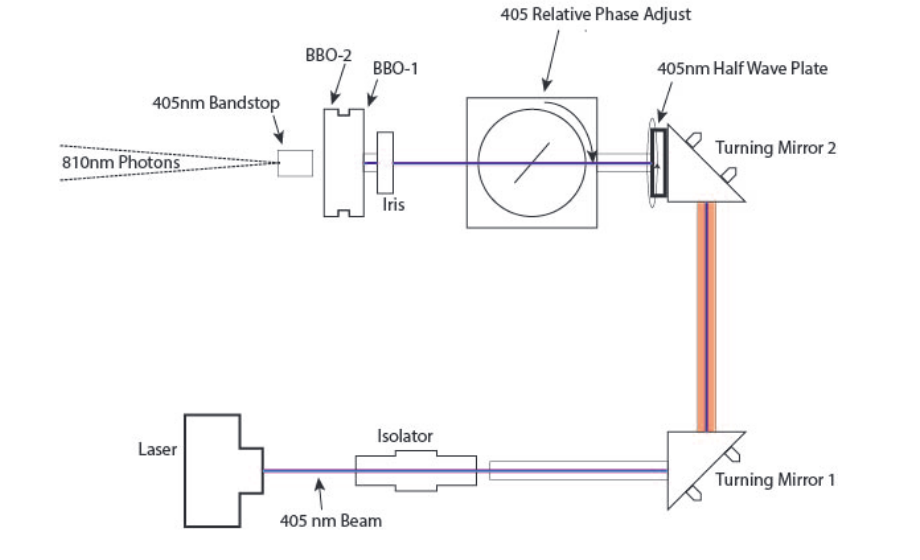
\includegraphics[scale=0.5]{images/laser-block.png}
			\caption{} 
			\label{laser-block}
		\end{subfigure}
		\begin{subfigure}{0.45\textwidth}
			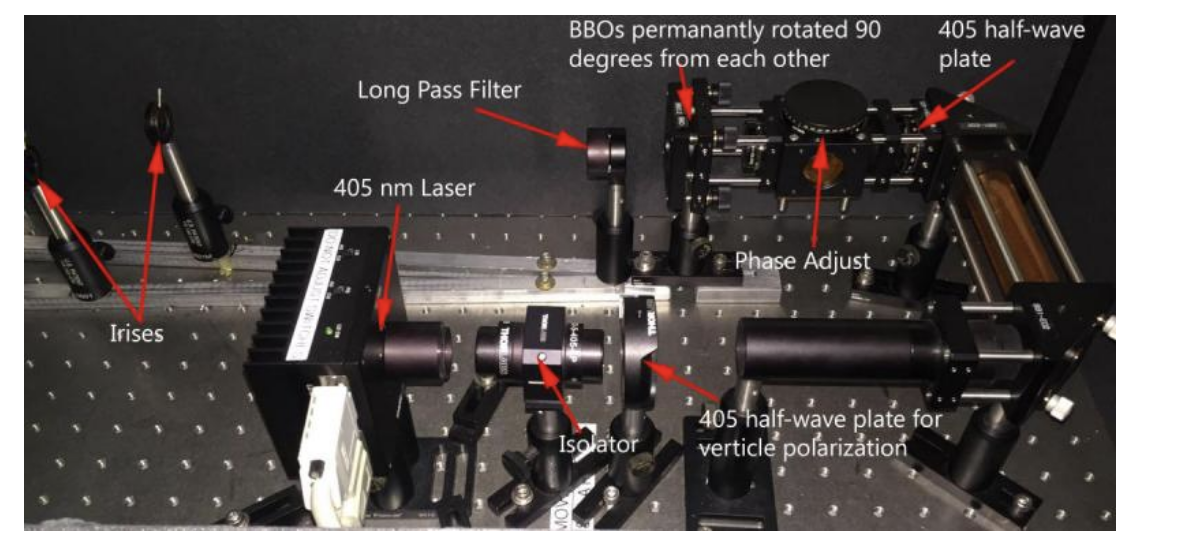
\includegraphics[scale=0.5]{images/laser-photo.png}	
			\caption{}
			\label{laser-photo}
		\end{subfigure}
		\caption{(a) Schematic diagram of the laser used in the experiment, along with the HWP and BBOs. The 405
			nm bandstop is not present in our experiment. (b) Image of the laser as it exists in our
			experimental setup. The long pass filter and irises were not used in our experiment. Both of these
		images were taken from \cite{manual}}
	\end{figure}

	A photo of the detector setup is shown in figure \ref{detector-photo}, 
	the detector portion of the apparatus consists of two detection arms, 
	with each arm having a HWP,
	a beam splitter, a long pass filter and a detector at the very end. The beam splitter is a clear cube
	which only lets through horizontally polarized light, and the long pass filter is used
	to only allow the entangled photons through, this will also become clear in the next section. 
	The signal from the detectors is then fed through
	to an APD, a device which measures coincidences (these are the \( N_{vv} \) quantities from the earlier
	section). In this experiment, the coincidences are measured as photons which arrive at both detectors
	within 5 nanoseconds of each other -- for most photons which arrive within this window, we can safely say
	that they originated from the same photon (before being split by the BBO), and thus are entangled. The
	size of 5 ns is chosen to account for slight differences in the beam paths and other potential sources of
	error. 
	\begin{figure}
		\centering
		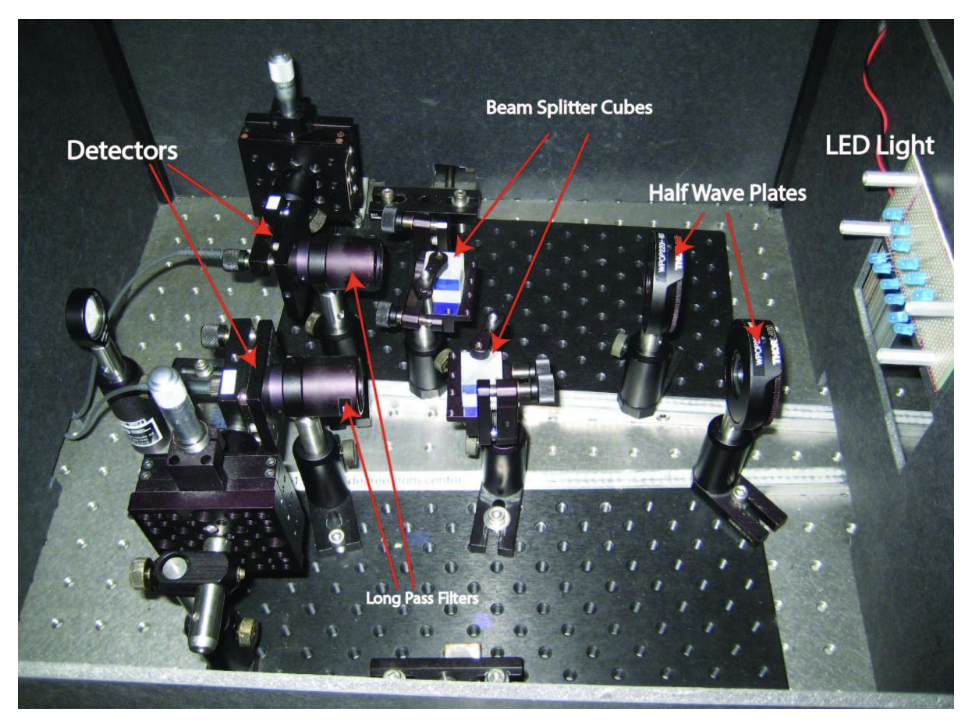
\includegraphics[scale=0.5]{images/detector-photo.png}
		\caption{Photo of the detector setup in our experiment. The laser beam comes in from the right, and
			interacts with the half wave plates, then the beam splitter cubes, before passing through the long
		pass filter then into the detector. This image was taken from \cite{manual}}  
		\label{detector-photo}
	\end{figure}

	The signal from the APDs is then fed to an FPGA, which is already pre-programmed to send the correct data
	to the LabVIEW application on the neighboring computer. From here, we can read off the values displayed
	on the monitor to collect our data. 

	\section{Procedure}

	For the experimental procedure, we will split this section into multiple parts. The actual experiment
	itself and the data collection is very easy -- all we will have to do is turn the HWPs to
	specific angles, turn on the laser, and read off the coincidences measured by the detector. Thus, a large
	part of this section will be dedicated to the \textit{calibration} of the setup, a process that occupied
	the vast majority of our time. 
	
	\subsection{Beam Alignment}
	
	\subsubsection{Violet Beam}

	To begin, the first section we work on is the first half of the apparatus, where the violet laser light
	is generated. Here, the first thing we need to make sure above all else is that the entangled pairs of
	photons are being generated properly. For us, that means we need to verify three things: first, the laser
	light is properly polarized before entering the HWP. Secondly, that the HWP angle is
	set to the correct angle to get an even distribution of vertical and horizontal pairs and finally, we
	need the entire beam path to be level, between the laser and detector. The first criterion
	is easy to verify: right after the laser passes through the linear polarizer, we use another piece of
	polarizing film to ensure that the beam is indeed polarized, which we do by rotating the film about the
	axis of light propagation. To explain how to calibrate the second criterion, it is first useful to
	understand the BBO plates and how they are set up.   

	As shown in figure \ref{laser-block} and \ref{laser-photo}, there are two BBOs in our experimental setup, 
	one vertical and one horizontal.
	The objective of the BBOs, as we mentioned earlier, is used to generate the entangled pairs, which is
	done by "splitting" a photon into two lower energy photons, but ones which have the same polarization as
	the original incoming photon. That is, the BBOs effectively give us this mapping:
	\[
		\ket*{V} \to \ket*{vv}
	\]
	Here, \( \ket*{V} \) is used to denote a higher energy particle, and \( \ket*{vv} \) is the two lower
	energy photons also with vertical polarization. Then, we can rotate one of the BBOs by \( 90^{\circ} \),
	so that we can also generate the horizontal photons:
	\[
		\ket*{H} \to \ket*{hh}
	\]
	Now, we can see why we needed the long pass filter on the detector end: because the entangled pairs are
	only present at lower energy, then in order to ensure that no other particles are being detected we
	remove them using the long pass filter. Furthermore, now that we know how the BBOs work, we can move on
	to the second calibration criterion. Recalling that we ultimately want to create a Bell state after the
	BBOs, it means that we require an equal portion of \( \ket*{vv} \) and \( \ket*{hh} \) pairs after the
	particles pass through the BBOs -- the only way to guarantee that is if we have an equal superposition of
	\( \ket*{V} \) and \( \ket*{H} \), so this motivates us to set the HWP to exactly \(
	22.5^{\circ} \) so that we get a rotation of exactly \( 45^{\circ} \), which gives us the state:
	\[
		\ket*{\psi} = \frac{1}{\sqrt{2}}(\ket*{vv} + \ket*{hh}) = \ket*{\Phi^{+}}
	\]
	as an output, which is exactly what we want. Finally, because there is a gap between the two BBOs, we
	introduce a small phase shift \( \delta \) to account for this: 
	\begin{equation}
		\label{exp-state}
		\ket*{\psi} = \frac{1}{\sqrt{2}}(\ket*{vv} + e^{i \delta}\ket*{hh})
	\end{equation}
	Finally, the last criterion is also relatively easy: there is a paper target mounted on the detector side
	of the experiment, so all we had to do was adjust the height of the laser until the light hit the center
	of the target. This step was actually complete when we found the experiment, so we didn't have to change
	anything for this portion.

	\subsubsection{Detector}

	Now, with the violet beam calibrated, we now move to calibrating the detector half of the experiment.
	Assuming that we made sure that the laser and detector reside on the same plane, the next thing to make
	sure is that the detectors are pointed directly at the output of the BBOs, so that the coincidences may
	be counted. 

	For this portion, we first took out the HWP, the beam splitter cubes and also the long pass
	filters. Then, to determine the beam path, we used a red laser and fed it optical fiber, so that the
	laser light would shine backwards toward the laser. This way, we can see the beam path more easily. We
	then use the adjusting knobs on the detectors to control the azimuthal and longitudinal angles, and the
	angle of the beam (we can adjust the detector arm altogether). Therefore, with all these degrees of
	freedom, it was much harder to find the perfect configuration than it actually seems. 

	When we had a configuration we thought was good enough, the way we tested it was to power on the laser,
	and look for the counts on the left side of the LabVIEW program. To do this, we had to place the
	long-pass filters back to cover the detectors, to protect them against the violet light. Because the long
	pass filters only filter out frequency (and leave polarization alone), we don't have to be \textit{too}
	careful with how we place these, so long as we don't touch any other part of the apparatus with it.
	If the raw counts were high on both arms (about 70,000 is what we aim for), then the detector was 
	calibrated properly.

	\subsection{Calibration}

	Now that the entire apparatus is aligned, the next thing we need to do is calibrate the HWPs, both the
	one in the box with the laser and the two in the box with the detector. Starting with the former, recall
	that we want this HWP to be rotated to exactly \( 22.5^{\circ} \) so that we get a state which is
	polarized at exactly \( 45^{\circ} \) before it passes through the BBOs. However, the fundamental issue
	with simply using the tick marks on the HWP is that it is not reliable, in the sense that a \( 0^{\circ}
	\) reading on the HWP does not correspond to the vertical. As such, we need another way to determine the
	optimal HWP angle, where we will make use of the LabVIEW program.   
	To do so, we remove the two HWPs in the detector box,
	but leave the beam splitting cubes in. Then, we turn on the laser, and turn the HWP until our coincidence
	counts are maximized. Because the horizontal counts are maximized, 
	this means that in its current configuration the
	laser is only outputting horizontally polarized light. Then, while we cannot trust the absolute reading,
	we will assume that the spacing between the tick marks can be trusted, so a rotation by \( \theta \) can
	be measured.   

	To check that we can trust the tick spacing, we can rotate the HWP by 45 degrees, corresponding to a
	rotation of \( 90^{\circ} \) meaning that the laser now only outputs \( \ket*{vv} \) states. Such a state
	is guaranteed to be deflected by the beam splitter, and as a result we should get a coincidence count of
	near zero. When we attempted this on our HWP, this is precisely what we see.    
	Now, returning to the angle which maximized the coincidence, we now proceed to turn the phase adjustment
	knob until the counts are maximized; if the coincidences were not already maximized, this process should
	increase the coincidence counts even further. This configuration for the HWP and phase adjustment were
	then recorded: the HWP's maximum was found at \( 27^{\circ} \pm 2^{\circ} \), and the phase was maximized at
	\( 308^{\circ} \pm 2^{\circ} \). The uncertainty here is determined by the smallest difference between
	two ticks, which was 2 degrees in both knobs.  

	Finally, the last thing to calibrate is the half wave plates in the detector box. Before we determining
	the offsets, it is useful to first verify that the HWPs on both detector arms work as we expect. To
	verify this, we turn the laser on, and rotate each HWP through a range of angles, recording their
	\textit{raw counts} (not coincidence counts) periodically. The raw counts are independently calculated
	for each HWP, so rotating one HWP should not affect the raw count of the other. 
	Because HWPs generate rotations and our measurements are projections, rotating the HWP through a range of
	angles and observing the raw counts amounts to rotating a vector around the unit circle and observe its
	projection on the \( x \)-axis -- essentially, we expect to observe a sinusoid curve. The data for 
	portion and corresponding plot are shown in \ref{count-table} and \ref{count-plot}, respectively. 
	From the plot, it is clear
	that a sinusoid is exactly what we observe, which gives good evidence that our HWPs operate as we expect.    

	\begin{figure}
		\centering
		\begin{subfigure}{0.45\textwidth}
			\begin{tabular}{|c|c|c|c|}
				\hline
				\textbf{$\theta_A$} & \textbf{Beam A counts} & \textbf{$\theta_B$} & \textbf{Beam B counts} \\ \hline
				0.5                                     & 65042                & -65                                     & 64426                \\ 
				20                                      & 42360                & -60                                     & 63434                \\
				40                                      & 7738                 & -40                                     & 31400                \\
				60                                      & 17432                & -20                                     & 4806                 \\
				80                                      & 56312                & 0                                       & 25706                \\
				100                                     & 60688                & 20                                      & 59530                \\
				120                                     & 23176                & 40                                      & 52033                \\
				140                                     & 5720                 & 60                                      & 14239                \\
				160                                     & 38100                & 80                                      & 9355                 \\
				180                                     & 66370                & 100                                     & 44214                \\ \hline
			\end{tabular}
			\caption{}
			\label{count-table}
		\end{subfigure}
		\begin{subfigure}{0.45\textwidth}
			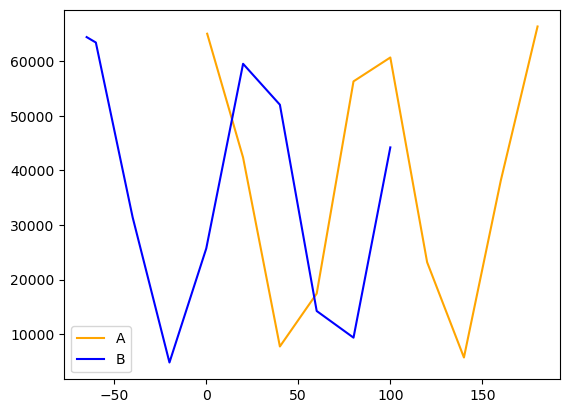
\includegraphics[scale=0.5]{images/contrast.png}	
			\caption{}
			\label{count-plot}
		\end{subfigure}
		\caption{(a) Table showing the counts for measurement beams A and B. (b) Plot of the count as a
			function of the angle \( \theta_{A, B} \). Linearly interpolating the lines was only done here
		for visual clarity only, so that we may see the sinusoidal pattern.}
	\end{figure}

	Now, we calibrate the HWPs and determine their offset. To do this, we 
	use the configuration derived from the previous paragraph that maximized the counts, and now adjust the
	HWPs on both arms until we recover the maximum coincidence count. In doing so, we are effectively
	finding the points on the HWP that are aligned with the \( \ket*{hh} \) basis -- mathematically, this is
	justified by the principle that the inner product is maximized when the two vectors are collinear, which
	is what we have here. We can then double check this is indeed the correct orientation, by rotating one
	of the HWPs by an additional \( 45^{\circ} \). Doing so, this changes the measurement basis to the \(
	\ket*{hv} \) basis, and as a result we should expect near zero counts -- this is precisely what we
	observe. We then recorded the offsets by reading the angle listed on the HWP at this maximum, which was
	\( 295^{\circ} \) for detector A and \( 1^{\circ} \) for detector B.  

	\subsection{Contrast}
	
	In this section, we will calculate a quantity called the contrast, which will allow us to essentially
	determine how ideal our current calibration has been. To do this, we calculate a quantity called the
	contrast, defined as follows:
	\[
		\text{contrast} = \frac{\max(\text{coincidences}) -
		\min(\text{coincidences})}{\max(\text{coincidences}) + \min(\text{coincidences})}
	\]
	In an ideal world, we should expect this value to equal 1. This is because the
	minimum count should be given when our measurement basis is \( \ket*{hv} \) or \( \ket*{vh} \), a
	measurement basis which matches neither of the two states we produce, 
	\( \ket*{vv} \) and \( \ket*{hh} \), and as such we should get a coincidence count of zero. We can then
	compute a contrast for each HWP, by fixing one while varying the other. Doing so, we get a value of 0.987 
	for detector A, and 0.978 for detector B. The reason
	they are not exactly 1 is due to experimental uncertainties, with one large contributor likely being the
	fact despite the room being dark we still obtain accidental coincidences. 
	However, the fact that they are extremely close to 1 gives good evidence that our half wave plates not
	only work as expected but the calibration of our system is indeed very good. 

	\section{Results and Analysis} 
	\subsection{Characterizing the Bell State}

	With the HWP contrast calculated, this concludes the last of our calibration, and we now move on to
	characterizing the Bell state we have produced. To do this, we follow the analysis steps in
	\cite{dehlinger}
	closely. Recall that if our HWP on the laser side acts as
	intended, then we produce the state given by equation \ref{exp-state}. In general however, because the
	HWP just generates a rotation, we can write the state after leaving the BBOs as: 
	\[
		\ket*{\psi_{DC}} = \sin \theta \ket*{hh} + e^{i \delta} \cos \theta \ket*{vv}
	\]
	where we rotated by an arbitrary amount \( \theta \), measured from the vertical. 
	Our goal is to solve for the value of \( \theta \) and the phase \( \delta \). 
	Given the state above, we can take its inner product with \( M(\alpha, \beta) \) 
	from equation \ref{projection}, which will yield the following probability:
	\begin{align*}
		P_{vv}(\alpha, \beta) &= |\sin \alpha \sin \beta \cos \theta + e^{i \delta}\cos \alpha \cos \beta \sin
		\theta|^2 \\
							  &= \sin^2 \alpha \sin^2\beta \cos^2 \beta + 2 \sin \alpha \sin \beta \cos \theta e^{i
		\delta}\cos \alpha \cos \beta \sin \theta + \cos^2 \alpha \cos^2 \beta \sin^2 \theta\\
		&= \sin^2 \alpha \sin^2 \beta \cos^2 \beta + \cos^2 \alpha \cos^2 \beta \sin^2 \theta +
		\frac{1}{4}\sin(2 \theta) \sin(2 \alpha) \sin (2 \beta) \cos \delta 
	\end{align*}
	we arrive at the last equation by taking the real part of \( e^{i \delta} \), probability is a real
	quantity. Now, we can then convert this probability into a count:
	\begin{equation}
		\label{count}
		N(\alpha, \beta) = A P_{vv}(\alpha, \beta) + C
	\end{equation}
	Here, the value of \( C \) exists in order to account for the number of accidental counts we will
	encounter in our experiment, and \( A \) refers to the total number of entangled pairs we generate. This
	equation should make sense, since \( N(\alpha, \beta) \) calculates the expected (in the probabilistic
	sense) number of coincidences we should get. Now, \cite{dehlinger} gives us the following relations:
	\begin{align*}
		C &= N(0^{\circ}, 90^{\circ}) \\ 
		A &= N(0^{\circ}, 0^{\circ}) + N(90^{\circ}, 90^{\circ}) - 2C 
	\end{align*}
	We can experimentally determine the counts, so we can determine \( C \) and \( A \) through experiment.
	Then, going back to equation \ref{count}, we can now use the experimentally determined values for \( A \)
	and \( C \) to solve for \( \theta \) and \( \delta \), using the following relations:
	\begin{align*}
		\tan^2 \theta &= \frac{N(90^{\circ}, 90^{\circ}) - C}{N(0^{\circ}, 0 ^{\circ} - C}\\
		\cos \delta &= \frac{1}{\sin(2 \theta)}\left( \frac{4(N(45^{\circ}, 45^{\circ}) - C}{A} - 1 \right) 
	\end{align*}
	We then perform these measurements, which are summarized in table \cite{dehlinger}. For each value of \( N \), we
	took 9 measurements, then computed the arithmetic mean to obtain a value for each \( N(\alpha, \beta) \).
	Then, solving for \( \theta \) and \( \delta \), we obtain:
	\[
		\theta = 43.6^{\circ} \pm 2^{\circ} \quad \delta = 37.5 \pm 2^{\circ}
	\]
	Here, we attach an error of \( 2^{\circ} \) to account for our uncertainty in the setting of our HWPs.
	In some sense, this is a more natural uncertainty to take than the propagated uncertainty, as it is a
	better representation of the potential variance in our measurements. 
	This leads to the state:
	\[
		\ket*{\psi_{DC}} = 0.72 \ket*{hh} + e^{i \delta} (0.68) \ket*{vv}
	\]
	Knowing that in the ideal case we have \( \theta = 45^{\circ} \), our experimental value of \( \theta =
	43.6^{\circ} \) indicates that our bell state is very nearly ideal (if not exactly ideal), 
	indicating that our calibration steps were done properly. The counts we observe here also match exactly
	what the mathematics tell us. For a perfect bell state, we have \( \theta = 45^{\circ} \) and \( \delta = 0 \), 
	so \( P_{vv}(\alpha, \beta) \) has a very nice interpretation:
	\[
		P_{vv}(\alpha, \beta) = \frac{1}{2}\cos^2(\beta - \alpha)
	\]
	meaning that the probability only depends on the difference between the two angles. Because the phase
	\( \delta \) doesn't change in our experiment, then this means that regardless of the value of \( \delta \),
	the probability should be constant and only a function of the difference \( \beta - \alpha \). In the
	context of our data, this means that \( N(0^{\circ}, 0^{\circ}), N(45^{\circ}, 45^{\circ}) \) and 
	\( N(90^{\circ}, 90^{\circ}) \) should all have similar values, and this is precisely what we see in
	table \cite{dehlinger}. 
	\begin{table}[]
		\centering
		\def\arraystretch{1.3}
		\begin{tabular}{|c|c|c|c|}
			\hline
			\( N(0^{\circ}, 0^{\circ}) \) & \( N(45^{\circ}, 45^{\circ}) \) & \( N(90^{\circ}, 90^{\circ})
			\)& \( N(0^{\circ}, 90^{\circ}) \)\\ \hline
			1464                                 & 1248               & 1324                                   & 18                \\
			1392                                 & 1280               & 1378                                   & 12                \\
			1480                                 & 1324               & 1252                                   & 24                \\
			1552                                 & 1234               & 1414                                   & 14                \\
			1486                                 & 1336               & 1384                                   & 18                \\
			1470                                 & 1236               & 1322                                   & 10                \\
			1500                                 & 1260               & 1358                                   & 18                \\
			1436                                 & 1182               & 1324                                   & 32                \\
			1418                                 & 1212               & 1250                                   & 28   \\ \hline            
		\end{tabular}
		\caption{Coincidence counts for different angle configurations of the measurement HWPs. Notice the
		similar values in \( N(0^{\circ}, 0^{\circ}), N(45^{\circ}, 45^{\circ}) \) and \( N(90^{\circ},
	90^{\circ}) \), which is behavior we expect.}
		\label{char-table}
	\end{table}

	\subsection{Calculating S}
	With the Bell state characterized, we are ready to move on to the final quantity to calculate, which is
	to calculate \( S \). Recall that earlier we introduced the CHSH inequality as the quantity \( S \):
	\[
		S = E(\alpha, \beta) - E(\alpha, \beta') + E(\alpha', \beta) + E(\alpha', \beta') \leq 2
	\]
	where each \( E(\alpha, \beta) \) is defined as:
	\[
		E(\alpha, \beta) = \frac{N_{vv} + N_{vh} - N_{hv} + N_{hh}}{N_\text{total}}
	\]
	So, now we define a measurement basis that maximizes \( S \). It should be noted that we need to be
	specific about which basis we choose, as not all \( \alpha, \alpha', \beta, \beta' \) values will violate
	\( |S| \leq 2 \). Following \cite{dehlinger}, we choose our angles \( \alpha = 0^{\circ}, \beta = 22.5^{\circ} \),
	and \( \alpha' = 45^{\circ}, \beta' = 67.5^{\circ} \) and measure the coincidence counts for each pair \(
	(\alpha, \beta), (\alpha', \beta), (\alpha, \beta'), (\alpha', \beta')\), which is summarized in table
	\ref{exp-data}. As for the uncertainties in our measured coincidences, we can derive the uncertainty by using the
	fact that the coincidence counting is a Poisson process, and thus the variance scales with \( \sqrt{N}
	\), where \( N \) is the count.   
	\begin{table}
    \def\arraystretch{1.2}
	\centering
    \begin{tabular}{|c|c|c|c|}
    \hline
    \multicolumn{1}{|l|}{\textbf{Angle pairs}}      & \textbf{Polarization A} & \multicolumn{1}{l|}{\textbf{Polarization B}} & \textbf{Coincidences} \\ \hline
    \multirow{4}{*}{($\alpha$, $\beta$)}   & 0                       & 22.5                                         & 1323.8                \\ \cline{2-4} 
                                           & 90                      & 22.5                                         & 268.8                 \\ \cline{2-4} 
                                           & 90                      & 112.5                                        & 1251.4                \\ \cline{2-4} 
                                           & 0                       & 112.5                                        & 321.2                 \\ \hline \hline
    \multirow{4}{*}{($\alpha$, $\beta'$)}  & 0                       & 67.5                                         & 190.2                 \\ \cline{2-4} 
                                           & 90                      & 67.5                                         & 1341.6                \\ \cline{2-4} 
                                           & 90                      & 157.5                                        & 186.4                 \\ \cline{2-4} 
                                           & 0                       & 157.5                                        & 1434.2                \\ \hline \hline
    \multirow{4}{*}{($\alpha'$, $\beta$)}  & 45                      & 22.5                                         & 1319.2                \\ \cline{2-4} 
                                           & 135                     & 22.5                                         & 334.4                 \\ \cline{2-4} 
                                           & 135                     & 112.5                                        & 1229.4                \\ \cline{2-4} 
                                           & 45                      & 112.5                                        & 268.8                 \\ \hline \hline
    \multirow{4}{*}{($\alpha'$, $\beta'$)} & 45                      & 67.5                                         & 1237.0                \\ \cline{2-4} 
                                           & 135                     & 67.5                                         & 414.2                 \\ \cline{2-4} 
                                           & 135                     & 157.5                                        & 1244.4                \\ \cline{2-4} 
                                           & 45                      & 157.5                                        & 373.2                 \\ \hline
    \end{tabular}
    \caption{Collected coincidences for the \( (\alpha, \beta) \) pairs described, which is then used to
		compute \( S \). For each coincidence we
	have, as it is modeled by a Poisson process, has an uncertainty of \( \sqrt{N} \), where \( N \) is the
number of coincidences we have.}
\label{exp-data}
\end{table}

	From here, it is easy to calculate \( S \), which we can compute by simply calculating \( E(\alpha,
	\beta)\) for each pair of angles, and sum them all to get \( S \). For our data, we obtain a value of \(
	S = 2.52 \pm 0.07 > 2\), so the CHSH inequality is violated. This allow us to conclude that hidden
	variable theories cannot be at play, since had they existed the value of \( S \) would be bounded. This
	is the ultimate result that we want to achieve, so this result concludes the experiment.    


	\section{Conclusion and Reflection}

	Overall, with the CHSH inequality violated, this indicates that our experiment was indeed successful in
	demonstrating that there are no hidden variable theories at play. In truth, while reproducing such a
	famous result in the lab is certainly rewarding, this lab certainly felt more frustrating than enjoyable
	at times particularly due to the amount of time we had to spend calibrating the device. Because of all
	the degrees of freedom we had to control, at times it felt like there were so many variables we had to
	keep track of that troubleshooting the source of an error was an immense challenge. 

	All in all, this lab really gave me a newfound respect for all the experimentation labs out there that
	use lasers and complex optical setups. In this context, our experimental setup is extremely simple: one
	laser, a couple of half wave plates and a detector is all that there is, and even such a simple setup
	took us \textit{days} to calibrate properly before we could measure a result. It really puts into context
	why these experiments are so sensitive to small deviations, and I can only imagine how difficult it is to
	"debug" the experiment. 

	Despite all this though, there are still some very fun parts of the lab that I take away: this was my
	first time working with a laser of this power which felt very cool, and also learning of the creative
	ways we calibrate our instruments (such as sending the red laser backwards through the detector and
	aiming it to align the beam path) was very interesting -- it makes me want to learn more about how
	calibration of larger setups are conducted.      
	 

	\nocite{*}
	\printbibliography



\end{document}
